\titledquestion{Tree Structure and Traversal}

\newcommand{\stack}[5]{
    \begin{minipage}{.13\linewidth}
        \begin{tikzpicture}[scale=0.5]
            \cell{#1}
            \cell{#2}
            \cell{#3}
            \cell{#4}
            \cell{#5}
        \end{tikzpicture}
    \end{minipage}
}

You should solve the below questions following these steps:
\begin{enumerate}
    \item Decide on an appropriate \textbf{data structure} to implement the traversal.
    \item When doing \textbf{Breadth First Traversal}, push children of a node into the data structure in alphabetical order.
    \item Consider \textbf{poping an entry} and \textbf{pushing all its children} as one step.
\end{enumerate}

\textbf{Example: }
Given a tree with root \textbf{A}: \\
\begin{figure}[h]
    \centering
    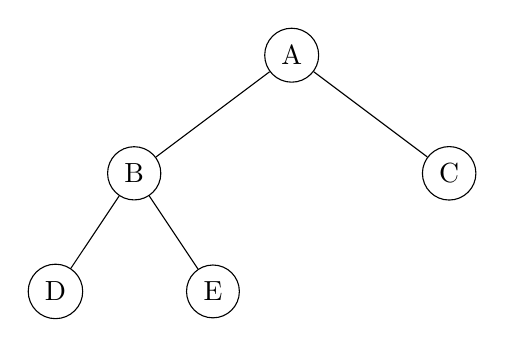
\begin{tikzpicture}[level distance=1.5cm,
        level 1/.style={sibling distance=4cm},
        level 2/.style={sibling distance=2cm},
        every node/.style = {draw, circle}]
        \node {A}
        child { node {B}
            child { node {D} }
            child { node {E} }
        }
        child { node {C} };
    \end{tikzpicture}
    \label{fig:example_pic}
\end{figure}

The process of doing \textbf{Breadth First Traversal} is: \\

\begin{figure}[h]
    \centering
    \stack{}{}{}{}{A} \to
    \stack{}{}{}{C}{B} \to
    \stack{}{}{E}{D}{C} \to
    \stack{}{}{}{E}{D} \to
    \stack{}{}{}{}{E} \to
    \stack{}{}{}{}{}
    \label{fig:example_sol}
\end{figure}

\pagebreak
\begin{parts}

    \part[5] Run \textbf{Breadth First Traversal} on the tree with root \textbf{A} and draw the whole process in the space below.

    \begin{figure}[h]
        \centering
        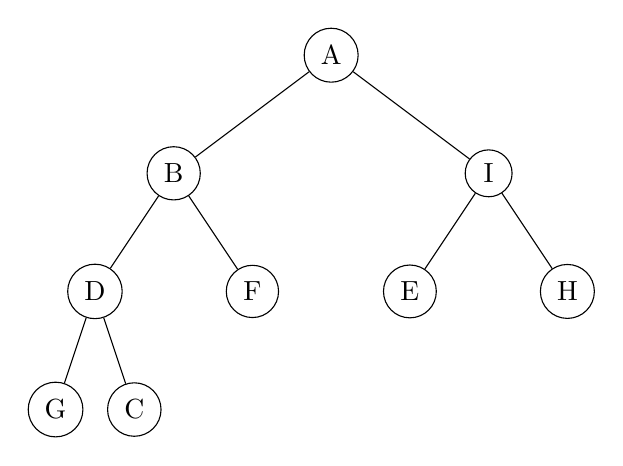
\begin{tikzpicture}[level distance=1.5cm,
            level 1/.style={sibling distance=4cm},
            level 2/.style={sibling distance=2cm},
            level 3/.style={sibling distance=1cm},
            every node/.style = {draw, circle}]
            \node {A}
            child { node {B}
                child { node {D}
                    child { node {G} }
                    child { node {C} }
                }
                child { node {F} }
            }
            child { node {I}
                child { node {E} }
                child { node {H} }
            };
        \end{tikzpicture}
        \label{fig:traversal_question_1}
    \end{figure}

    \begin{solution}
        \vspace{30em}
    \end{solution}

    \pagebreak
    \part[5] Run \textbf{Pre-order Depth First Traversal} on the tree with root \textbf{A} and draw the whole process in the space below.

    \begin{figure}[h]
        \centering
        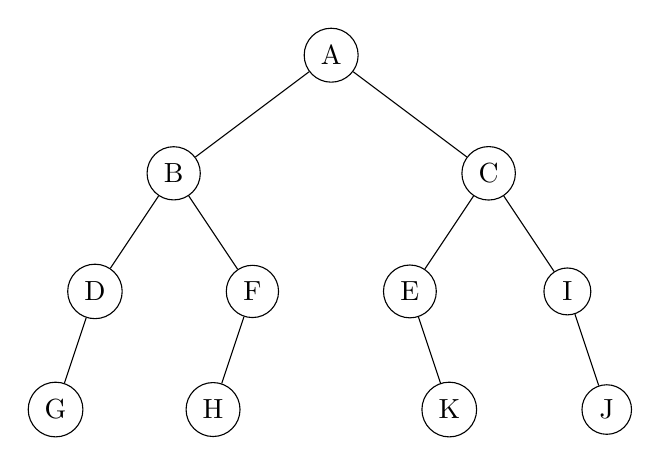
\begin{tikzpicture}[level distance=1.5cm,
            level 1/.style={sibling distance=4cm},
            level 2/.style={sibling distance=2cm},
            level 3/.style={sibling distance=1cm},
            every node/.style = {draw, circle}]
            \node {A}
            child { node {B}
                child { node {D}
                    child { node {G} }
                    child { edge from parent[draw=none] }
                }
                child { node {F}
                    child { node {H} }
                    child { edge from parent[draw=none] }
                }
            }
            child { node {C}
                child { node {E}
                    child { edge from parent[draw=none] }
                    child { node {K} }
                }
                child { node {I}
                    child { edge from parent[draw=none] }
                    child { node {J} }
                }
            };
        \end{tikzpicture}
        \label{fig:traversal_question_2}
    \end{figure}

    \begin{solution}
        \vspace{30em}
    \end{solution}

    \pagebreak
\end{parts}